%!TEX root = main.tex

\newpage
\section{문서 작성 시작하기}
\label{sec:text}
\subsection{예시 코드 구경하기}
그럼 지금부터는 본격적으로 문서 작성을 시작해 보도록 하겠습니다.
사실 진짜 기본적인 내용은 \ref{sec:beginning}장에서 모두 끝났기 때문에, 지금부터는 \lt 의 각 기능들을 어떻게 활용하는지에 초점을 맞추어 살펴보도록 하겠습니다. 아마 여기도 예시를 들어 설명하는 것이 보다 이해가 쉬울 겁니다. 간단한 예시 코드를 보도록 하죠.
\begin{Verbatim}[frame=single]
\documentclass{article}
\usepackage{kotex}
\usepackage[left=2.5cm,right=2.5cm,top=3cm,bottom=3cm,a4paper]{geometry}
\author{KSAstudent}
\date{\today}
\title{이게 레이텍입니다}
\begin{document}
    \maketitle
    \tableofcontents
    \vspace{3cm}
    \section{글 작성하기}
    \label{sec:intro}

        \subsection{기본적인 글}
        \label{sec:text}
        그냥 적으면 됩니다. ㅎㅎ
        
        \subsection{그림 넣기}
        \label{sec:image}
        \begin{center}
          \emph{뒤에서} 설명드릴게요.
        \end{center}

    \section{수식 작성하기}
    \ref{sec:image}와 크게 다르지 않습니다.\\
    뒤에서 설명드릴게요.

\end{document}
\end{Verbatim}
이 코드의 결과물은 다음 페이지에서 확인하실 수 있습니다.

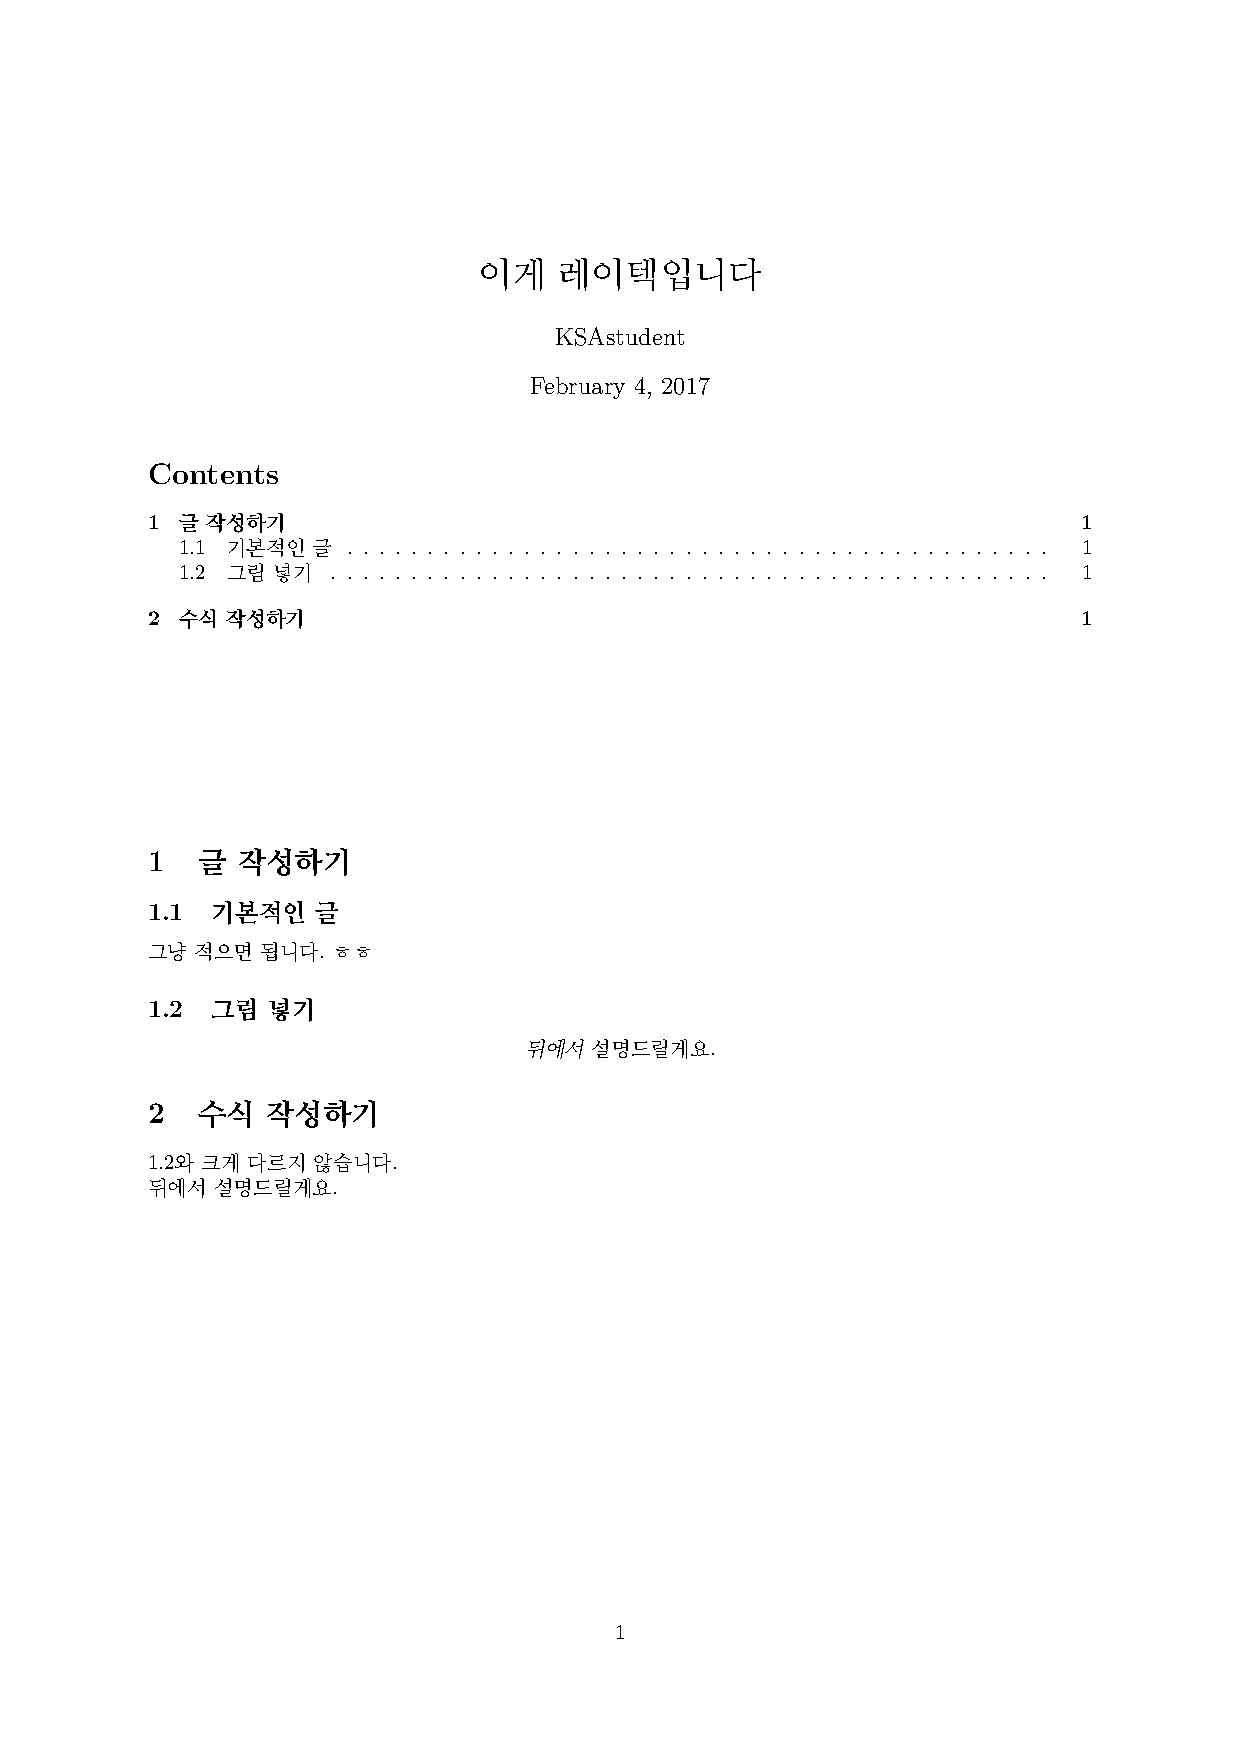
\includepdf[fitpaper=true]{example/examplepdf.pdf}

이해하셨나요? 지금부터 천천히 하나씩 살펴봅시다.

\subsection{글의 구조}
\label{sec:text-org}
일단 글의 전체적인 구조부터 파악해 봅시다.
앞서 \ref{preamble}장에서 preamble에 대한 설명을 들으셨을 겁니다.
\verb|\documentclass| 부터 \verb|\begin{document}| 까지가 preamble에 속합니다.
그 아래 \verb|\begin{document}|부터 \verb|\end{document}|까지는 글의 실질적인 내용에 속하죠.

글의 내용을 천천히 살펴봅시다.
여기서 사용된 article 이라는 class는 section부터 시작해 subsection, subsubsection, paragraph 순으로 이어지는 문서 구조를 가지고 있습니다.
첫 번째 section의 첫 번째 subsection은 1.1, 두 번째 subsection은 1.2, ... 이런 식으로 구조화가 이루어지는 거죠.
앞서 말씀드렸듯이 \verb|\begin{}|과 \verb|\end{}|는 다양한 용도로 사용됩니다.
\verb|\begin{}|과 \verb|\end{}|사이를 하나의 환경, envorinment라고 부르는데, 여기서는 center라는 envorinment를 정의하기 위해 사용되었죠.
특정 environment안의 글들은 그 environment의 특징을 띄게 됩니다.
여기서 center라는 environment는 글을 가운데 정렬하는 역할을 합니다.

거의 대부분의 \lt 코드들은 본질적으로  위 코드와 크게 다르지 않습니다.
environment안에 environment가 있다거나 하는 복잡한 구조라도, 펼쳐놓고 보시면 이걸로도 충분히 이해하실 수 있습니다.

\subsection{Preamble의 기능}
\label{sec:text-preamble}
그렇다면 지금부터는 아까 설명드린 preamble 각 줄이 어떤 역할을 하는지 보다 구체적으로 살펴보도록 하겠습니다.
사실 제가 예시로 든 것 말고도 수많은 package나 기능들이 있지만, 일단 그것들이 어떤 식으로 사용되는지 이해해 보시라는 의미에서 몇 가지 자주 쓰일만한 것들만 예시로 넣었습니다.
\begin{itemize}
  \item 우선 맨 첫줄의 \verb|\documentclass|에 대한 설명은 \ref{documentclass}장에서 충분히 했으니 다음 줄부터 설명하겠습니다. 다양한 document class들은 나중에 하나씩 살펴보도록 하고요.

  \item \verb|\usepackage{kotex}|는 \ref{sec2-package}장에서 잠깐 언급했지만, 한글을 사용하기 위해 사용되는 package입니다. 이 package 없이는 한글이 제대로 표시되지 않죠.

  \item 다음 줄의 \verb|\usepackage[...]{geometry}| 부분을 살펴보도록 하겠습니다. \verb|\usepackage{geometry}|는 geometry라는 이름의 package를 사용하겠다는 명령이고, 사이에 있는 대괄호는 그 geometry라는 package를 어떻게 사용할 것인지, 옵션을 지정하는 부분입니다. Geometry라는 이름에서, 그리고 옵션의 내용에서 짐작하실 수 있듯이 이 package는 문서의 여백을 설정할 수 있는 package입니다. 사실 굳이 지정을 안하셔도 \lt 는 기본 설정대로 예쁜 문서를 만들어 줍니다. 그렇지만 문제가 있다면 여백이 조금 넓다는 거죠. 직접 한 번 해 보시면 아실 겁니다. 사실 이 여백은 어떻게 하면 가장 읽기 편한 문서를 만들 수 있을지, 다양한 방면에서 고려해 결정된 것이라곤 합니다. 그렇기에 저도 저 혼자 볼 문서는 기본 설정대로 만드는 경우가 많고요. 그렇지만 솔직히 여백이 너무 넓으면 부담스러운 경우가 많지 않습니까. 그럴 땐 이 패키지를 쓰시면 됩니다.
    
  \item 다음 세 줄은 연달아 author, date, title을 지정했네요. 별 거 없습니다. 말 그대로 지정한 거죠. 몇 줄 내려가 \verb|\begin{document}|아래에 \verb|\maketitle|이 보이시나요? 거기서는 여기서 지정한 값들을 바탕으로 제목을 만들어 줍니다. 아, \verb|\today|는 뭐냐고요? date 자리에 오늘 날짜를 자동으로 입력해 주는 명령어입니다. 굳이 \verb|\today|를 쓰지 않고 그냥 아무거나 넣으면 날짜 자리에 그게 뜰겁니다. 
\end{itemize}

이 코드의 preamble은 이게 전부입니다. 간단하죠?
이 코드에서 사용된 것 말고도  preamble에서는 다양한 일을 할 수 있습니다.
앞서 \ref{sec:1.2-ext}장에서 잠깐 언급했지만 새로운 명령을 정의해서 사용한다거나, 명령들이 어떻게 작동할지 구체적으로 설정하는 것도 가능합니다.
몇 가지는 뒤에서 천천히 소개하겠습니다.


\subsection{명령어 알아보기}
\label{sec:text-cmd}
지금부터는 \lt 의 명령어들을 구체적으로 알아보겠습니다.
사실 명령어라고 거창하게 이름 붙일 것도 없습니다.
앞에서 눈치채셨겠지만 \lt 는 \verb|\|로 시작하는 단어를 인식하고, 이는 모두 명령어라고 불리기 때문입니다.
잠시 \ref{sec:text-preamble}장 에서 자세히 살펴보지 않은 유용한 \lt 명령어들을 몇 가지 살펴보도록 하겠습니다.

우선 \verb|\maketitle|은 앞에서 설명드렸으니 그 다음 \verb|\tableofcontents| 부터 살펴보도록 하겠습니다.
예상하셨겠지만, \verb|\tableofcontents|는 문서의 목차를 만들어 줍니다.
앞서 설명했듯 \verb|\section|, \verb|\subsection|등을 이용하여 문서를 구조화시켜놓았다면 따로 별다른 설정을 하지 않아도 \verb|\tableofcontents| 명령어 하나로 그럴듯한 목차를 만들어 줄 겁니다.
물론 목차 생성의 설정을 바꾸는 것도 가능합니다만, 여기서는 깊게 다루지 않도록 하겠습니다.

다음으로 보이는 명령어는 \verb|\vspace{3cm}| 이네요.
이건 바로 알아보시지 못하셨을지도 모르겠네요.\\
\verb|\vspace| 란 vertical space의 줄임말로, 세로 여백을 조절할 수 있는 명령어입니다.
괄호 속의 3cm은 3cm의 여백을 두겠다는 의미죠.
센티미터 말고도 인치와 같은 다른 단위들을 사용하는 것도 가능합니다.
비슷한 방식으로 \verb|\hspace| 명령어는 가로 방향 빈칸을 두기 위한 명령어로 사용됩니다.

다음은 \verb|\section{글 작성하기}| 아래의 \verb|\label{sec:text}|를 봅시다.
label은 상호 참조를 위해 사용되는 명령어입니다.
글 작성하기라는 section을 뒤에서 참조하기 위해 이름을 붙여놓은 거죠.
이는 뒤에서 \verb|\ref{}|명령어와 함께 사용됩니다.
\verb|\ref{sec:image}|라는 명령어를 통해서 \verb|\label{sec:text}|를 불러온거죠.
여기서는 알아보지 못하시겠지만 이는 원하는 부분으로 하이퍼링크를 걸어줌과 함께 자동으로 번호를 매겨줍니다.
이 \lt 의 상호 참조 기능은 중간에 section, subsection을 추가하면 새롭게 번호가 매겨지기 때문에 무척 편리하고, 보다 구조화된 문서를 작성하는 데 도움이 됩니다.
물론 section, subsection 등에만 활용이 제한되어 있지 않고, 수식, 그림 등 다양한 부분에 사용 가능합니다.

마지막으로는 \verb|\emph{}| 명령어를 구경해 봅시다.
우리가 문서의 특정한 부분에 특정한 효과를 적용하고 싶다면 위에서 언급한 \verb|\begin{center}|, \verb|\end{center}|와 같이 environment를 이용할 수 있습니다.
그렇지만 한 단어나, 한 글자와 같은 보다 짧은 구간에 적용되는 효과의 경우 일반적인 \verb|\begin|, \verb|\end|로 구성되는 방식 대신 \verb|\emph|와 같은 방식이 사용되는 경우가 많습니다.
예상하실 수 있으시겠지만 emph 는 emphasis 를 줄인 표현으로, 단어를 강조할 때 사용됩니다. 영문의 경우 이 명령어를 사용할 경우 \emph{emphasis}와 같이 이탤릭체로 표현이 되지만, 한글과 한자의 경우 본래 이탤릭체가 없기 때문에\footnote{워드프로세서의 이탤릭 기능은 단순히 글자를 찌그러트린 것에 불과합니다. 실제로 한글이 이탤릭체를 지원하려면 이탤릭체가 포함된 한글 폰트가 필요합니다만, 영어와 달리 한글은 이탤릭체가 예쁘지도 않고, 전통적으로 사용되어 오지 않았기 때문에 이를 지원하는 한글 폰트는 거의 없다시피 합니다.} \emph{강조} 와 같은 형태로 나타나게 됩니다.

\subsection{문제가 생기셨나요??}
\label{sec:text-help}
여기서는 위에서 언급한 것과 같은 기본적인 문서 작성 과정에서 문제가 발생했을 시 대처할 수 있는 몇 가지 방법 및 주의 사항에 대해 언급해 드리겠습니다.
\begin{itemize}
\item tableofcontents, reference 와 같은 기능들은 올바르게 작동하기 위해 두 번의 컴파일이 필요할 수 있습니다. citation 기능을 사용할 경우에는 tex engine을 바꿔 가며 순서에 맞게 컴파일할 필요가 있기도 합니다만 여기서는 자세히 언급하지 않겠습니다. 물론 TeXStudio와 같은 프로그램을 사용하면 간단하게 해결할 수 있는 문제이기는 합니다. 어쨌든 목차나 reference 기능이 올바로 작동하지 않더라도 너무 걱정하지 마시고 한번 더 컴파일을 해 보세요.
\item 위에서 언급했듯이 \lt 는 environment의 중첩 사용을 허용합니다. 즉 environment 안에 environment가 들어갈 수 있습니다. 그러나 이 때 environment는 그 중첩 순서가 맞아야 합니다. 다시 말해
\begin{Verbatim}
\begin{environmentA} \begin{environmentB} \end{environmentB} \end{environmentA}
\end{Verbatim}
  는 허용되지만
\begin{Verbatim}
\begin{environmentA} \begin{environmentB} \end{environmentA} \end{environmentB}
\end{Verbatim}
  는 허용되지 않습니다.
\item \lt 의 모든 명령어는 대소문자를 구분합니다. 꼭 유의하세요. 그리고 명령어의 기준은 \verb|\|이 시작될 때부터 알파벳이 아닌 문자가 올 때까지 입니다. 다시 말해 명령어를 모두 입력하고 나면 빈 칸을 추가해 주어야 \lt 이 명령어가 끝났다는 점을 인식할 수 있습니다. 그렇지 않으면 없는 명령어를 사용했다며 에러를 배출하겠죠. 또한 새로운 명령어를 만들 때, 숫자나 괄호가 들어가는 명령어를 사용할 수도 없습니다.

\end{itemize}

%%% Local Variables:
%%% mode: latex
%%% TeX-master: "main"
%%% End:
